\chapter{Testi}
Testi tika sadalīti vairākās daļās, lai pārliecinātos par atsevišķu apakšsistēmu funkcionalitāti. Visi testi izriet no specifikācijas, lai pārbaudītu sistēmu atbilstību. Testi ietver darba punkta iestatīšanu RF jaudas pastiprinātājam, digitālās loģikas barošanas risinājuma novērtējumu, jaudas detektora elektrisko parametru noteikšanu pie 7.2 GHz un tīkla vadību ar TCP protokolu. Testos tiek izmantotas tādas mēriekārtas kā Metex M-3604D digitālais rokas multimetrs \cite{metex_multimeter}, Fluke 87 digitālais multimetrs \cite{fluke_multimeter}, SIGLENT SDS-1104X-U osciloskops \cite{oscil}, Rohde\&Schwarz signāla ģenerators SMP04 \cite{rs_signal_generator}, Rohde\&Schwarz VNA ZVK \cite{rs_vna}, BaseTech BT-305 barošanas avots \cite{test_powersupply} un IGENT SPL 1020 XE 200W DC programmējamo slodzi \cite{programmable_load}.
Testa sadaļās:
\begin{itemize}
    \item Darba punkta iestatīšanas/attiestatīšanas.
    \item 5 un 9 V barošanas risinājuma novērtējums.
    \item Jaudas detektora un koaksiāļo kabeļu novērtējums.
    \item Sistēmas vadība caur tīklu.
\end{itemize}

\section{HPA darba punkta iestatīšana/atiestatīšana}
Darba punkta noteikšanai (skat. 3.1. att.) tika mērīta noteces strāva , 12  un 24 V industriālā barošanas avota līnijas, ieslēgšanas/izslēgšanas slēdža vadības signāls un RF jaudas pastiprinātāja aizvara spriegums. Noteces strāva jaudas pastiprinātājam tiek mērīta ar multimetru, bet pārējie sistēmas parametri - ar osciloskopu.
\begin{figure}[H]
	\centering
    \includegraphics[width=0.8\textwidth]{pictures/test_diagram.png}\hspace{1cm}
    \caption{Darba punkta iestatīšanas/atiestatīšanas testa diagramma}
\end{figure}
Visās oscilogrammās 1. kanāls ir 12 V līnija, 2. kanāls ir 24 V līnija, 3. kanāls ir ieslēgšanas/izslēgšanas vadības signāls un 4. kanāls ir RF jaudas pastiprinātāja aizvara spriegums.
\begin{figure}[H]
	\centering
    \includegraphics[width=0.9\textwidth]{pictures/device_startup.png}\hspace{1cm}
    \caption{Sistēmas ieslēgšana}
\end{figure}
 3.2. att. ieslēdzoties sistēmai, tiek ieslēgts 12 V barošanas avots, kas nodrošina jaudu visiem 9 V un 5 V patērētājiem, tālāk jaudas pastiprinātāja aizvara spriegums tiek iestatīts uz -5 V, lai to aizvērtu. 24 V barošanas avots netiek ieslēgts, jo to dara  mikrokontrolleris ar manuālu vai tīkla komandu, tāpēc arī nevar novērot 24 V vadības spriegumu ieslēgšanas/izslēgšanas slēdzim.
\begin{figure}[H]
	\centering
    \includegraphics[width=0.9\textwidth]{pictures/load_nocap.png}\hspace{1cm}
    \caption{Sistēmas ieslēgšanās oscilogramma ar testa lauktranzistoru}
\end{figure}
\begin{figure}[H]
	\centering
    \includegraphics[width=0.9\textwidth]{pictures/capacitive_load.png}\hspace{1cm}
    \caption{Sistēmas ieslēgšanās oscilogramma ar testa lauktranzistoru un filtra kondensatoru}
\end{figure}
3.3. un 3.4. attēlā var redzēt darba punkta iestatīšanu, kur 3.4 attēlā tiek simulēts pats RF pastiprinātājs, pieliekot klāt kondensatorus filtrs. Kad tiek saņemta starta komanda mikrokontrollerī, tad tiek ieslēgts 24 V barošanas avots, kur momentā tiek nodrošināts aizvara spriegums ieslēgšanas/izslēgšanas p-kanāla lauktranzistoram, lai tas būtu aizvērtā stāvoklī. Tad pēc pāris milisekundēm tiek atvērts lauktranzistors un pēc datu lapas nodrošināta vismaz 100 milisekunžu aizture pēc p-kanāla lauktranzistora aktivizēšanas, lai nostabilizētos pārējie procesi.
\begin{figure}[H]
	\centering
    \includegraphics[width=0.9\textwidth]{pictures/load1load2_f.jpg}\hspace{1cm}
    \caption{Noteces strāvas kreisajam un labajam plecam RF jaudas pastiprinātājam}
\end{figure}
3.5. attēlā var redzēt noteces strāvas abiem RF jaudas pastiprinātāja pleciem. Kreisajā pusē 2.98 A tiek nodrošināti testa tranzistoram bez kapacitatīvas slodzes un labajā pusē 2.95 A ar kapacitatīvu slodzi, kas simulē RF jaudas pastiprinātāju.
\begin{figure}[H]
	\centering
    \includegraphics[width=0.9\textwidth]{pictures/load_off_nocap.png}\hspace{1cm}
    \caption{Sistēmas izslēgšana oscilogramma ar testa lauktanzistoru}
\end{figure}
\begin{figure}[H]
	\centering
    \includegraphics[width=0.9\textwidth]{pictures/cap_load_off.png}\hspace{1cm}
    \caption{Sistēmas ieslēgšanās oscilogramma ar testa lauktanzistoru un filtra kondensatoru}
\end{figure}
3.6. un 3.7. att. var redzēt sistēmas izslēgšanās procesu. Kad tiek saņemta komanda mikrokontrollierī par sistēmas atslēgšanu, tad RF jaudas pastiprinātājam tiek aizvērts, un pēc 100 milisekundēm aizvērts ieslēgšanas / izslēgšanas slēdzis un izslēgts 24 V industriālais barošanas avots.
\begin{figure}[H]
	\centering
    \includegraphics[width=0.8\textwidth]{pictures/test_diagram4.png}\hspace{1cm}
    \caption{Darba punkta iestatīšanas/atiestatīšanas testa diagramma ar differenciālo pāri}
\end{figure}
3.8. att. 1. un 2. kanāls veido diferenciālo pāri, kur tiek mērīts šunta rezistora sprieguma kritums, 3. kanāls mēra vadības signālu ieslēgšanas/izslēgšanas slēdzim un 4. kanāls aizvara spriegumu jaudas pastiprinātājam.
\begin{figure}[H]
	\centering
    \includegraphics[width=0.9\textwidth]{pictures/current.png}\hspace{1cm}
    \caption{Sprieguma krituma noteikšana uz šunta rezistora}
\end{figure}
 Osciloskopam mazākajā mērīšanas diapazonā ir mazāki kanāla trokšņi, tāpēc osciloskopa tausti tika iestatīti uz 10x un osciloskopā nokonfigurēts uz 1x, lai varētu mērīt lielāku signālu ar mazāku sprieguma diapazonu, bet, neskatoties uz to, 1V mērīšanas diapozonam ir 100 mV pk-pk troksnis, tādēļ nebija iespējams izmērīt 22 mV sprieguma kritumu uz šunta rezistora, bet, kad beidzas pārejas process, tad var redzēt, ka troksnis sāk svārstīties ap citu vērtību, bet tas nedod noteiktu vērtību.
\section{Elektrobarošanas plates testi}
Testā tika novērtēts iekārtu jaudas patēriņš un elektrobarošanas risinājuma novērtējums.
\begin{figure}[H]
	\centering
    \includegraphics[width=0.9\textwidth]{pictures/test_diagram2.png}\hspace{1cm}
    \caption{9 un 5 V barošanas testa diagramma}
\end{figure}
3.9. att. redzams testa iekārtu slēgums elektriski principiālajā ķēdē un slodzes pieslēguma vieta.
\begin{table}[H]
\captionsetup{singlelinecheck=off, justification=raggedleft}
\caption{9 V elektrobarošanas}
\centering
\begin{tabular}{|c|c|c|c|c|c|}
\hline
\multicolumn{2}{|c|}{\makecell{Ieejas parametri}} 
& \multicolumn{2}{c|}{\makecell{Izejas parametri}} 
& \multirow{2}{*}{\makecell{Slodze, \si{\ohm}}} 
& \multirow{2}{*}{\makecell{Eff, \%}} \\
\cline{0-3}
\makecell{Spriegums, \si{\volt}} 
& \makecell{Strāva, \si{\ampere}}
& \makecell{Spriegums, \si{\volt}}
& \makecell{Strāva, \si{\ampere}}
&  &\\ 
\hline
12.04\pm0.12 & 0.02\pm0.01 & 8.95\pm0.01 & 0.01\pm0.00 & 14280.00\pm0.00 & 37.16 \\ 
\hline
12.06\pm0.12 & 0.12\pm0.01 & 8.96\pm0.01 & 0.10\pm0.00 & 90.14\pm0.00 & 61.91 \\ 
\hline
12.02\pm0.12 & 0.22\pm0.01 & 8.96\pm0.01 & 0.20\pm0.00 & 44.84\pm0.00 & 67.76 \\ 
\hline
12.03\pm0.12 & 0.32\pm0.02 & 8.98\pm0.01 & 0.30\pm0.00 & 29.90\pm0.00 & 69.98 \\ 
\hline
12.03\pm0.12 & 0.42\pm0.02 & 8.98\pm0.01 & 0.40\pm0.00 & 22.44\pm0.00 & 70.09 \\ 
\hline
12.00\pm0.12 & 0.53\pm0.02 & 8.99\pm0.01 & 0.50\pm0.00 & 17.96\pm0.00 & 70.68 \\ 
\hline
11.99\pm0.12 & 0.63\pm0.02 & 8.99\pm0.01 & 0.60\pm0.00 & 14.98\pm0.00 & 71.40 \\ 
\hline
11.98\pm0.12 & 0.73\pm0.02 & 9.00\pm0.01 & 0.70\pm0.00 & 12.85\pm0.00 & 72.04 \\ 
\hline
11.98\pm0.12 & 0.83\pm0.02 & 9.00\pm0.01 & 0.80\pm0.00 & 11.25\pm0.00 & 72.41 \\ 
\hline
11.97\pm0.12 & 0.93\pm0.03 & 9.00\pm0.01 & 0.90\pm0.00 & 10.01\pm0.00 & 72.76 \\ 
\hline
11.96\pm0.12 & 1.03\pm0.03 & 9.00\pm0.01 & 1.00\pm0.00 & 8.99\pm0.00 & 73.06 \\ 
\hline
\end{tabular}
\end{table}

Izveidotais 9 V pārveidotāja risinājums spēj nodrošināt nepieciešamo jaudu slodzei.

\begin{table}[H]
\centering
\captionsetup{singlelinecheck=off, justification=raggedleft}
\caption{5 V elektrobarošanas}
\begin{tabular}{|c|c|c|c|c|c|}
\hline
\multicolumn{2}{|c|}{\makecell{Ieejas parametri}} 
& \multicolumn{2}{c|}{\makecell{Izejas parametri}} 
& \multirow{2}{*}{\makecell{Slodze, \si{\ohm}}} 
& \multirow{2}{*}{\makecell{Eff, \%}} \\
\cline{0-3}
\makecell{Spriegums, \si{\volt}} 
& \makecell{Strāva, \si{\ampere}}
& \makecell{Spriegums, \si{\volt}}
& \makecell{Strāva, \si{\ampere}}
&  &\\ 
\hline
8.95\pm0.01 & 0.02\pm0.01 & 5.15\pm0.01 & 0.01\pm0.00 & 13020.00\pm0.00 &  28.61 \\ 
\hline
8.96\pm0.01 & 0.11\pm0.01 & 5.15\pm0.01 & 0.10\pm0.00 & 51.22\pm0.00 & 52.02 \\ 
\hline
8.96\pm0.01 & 0.21\pm0.01 & 5.16\pm0.01 & 0.20\pm0.00 & 25.70\pm0.00 & 54.50 \\ 
\hline
8.98\pm0.01 & 0.31\pm0.02 & 5.16\pm0.01 & 0.30\pm0.00 & 17.19\pm0.00 & 55.37 \\ 
\hline
8.98\pm0.01 & 0.41\pm0.02 & 5.16\pm0.01 & 0.40\pm0.00 & 12.89\pm0.00 & 56.10 \\ 
\hline
8.99\pm0.01 & 0.51\pm0.02 & 5.16\pm0.01 & 0.50\pm0.00 & 10.31\pm0.00 & 56.28 \\ 
\hline
8.99\pm0.01 & 0.61\pm0.02 & 5.16\pm0.01 & 0.60\pm0.00 & 8.59\pm0.00 & 56.42 \\ 
\hline
9.00\pm0.01 & 0.71\pm0.02 & 5.15\pm0.01 & 0.70\pm0.00 & 7.35\pm0.00 & 54.87 \\ 
\hline
9.00\pm0.01 & 0.81\pm0.02 & 5.14\pm0.01 & 0.80\pm0.00 & 6.43\pm0.00 & 56.52 \\ 
\hline
9.00\pm0.01 & 0.91\pm0.03 & 5.15\pm0.01 & 0.90\pm0.00 & 5.72\pm0.00 & 56.60 \\ 
\hline
9.00\pm0.01 & 1.01\pm0.03 & 5.15\pm0.01 & 1.00\pm0.00 & 5.14\pm0.00 & 56.66 \\ 
\hline
\end{tabular}
\end{table}

Izveidotais 5 V pārveidotāja risinājums spēj nodrošināt nepieciešamo jaudu slodzei. Slēdzot to kaskādes slēgumā pēc 9 V elektrobarošanas avota, tiek paaugstināta lineārā sprieguma efektivitāte, jo ir mazāk jaudas jāizkliedē uz sevis.

\begin{figure}[H]
\centering
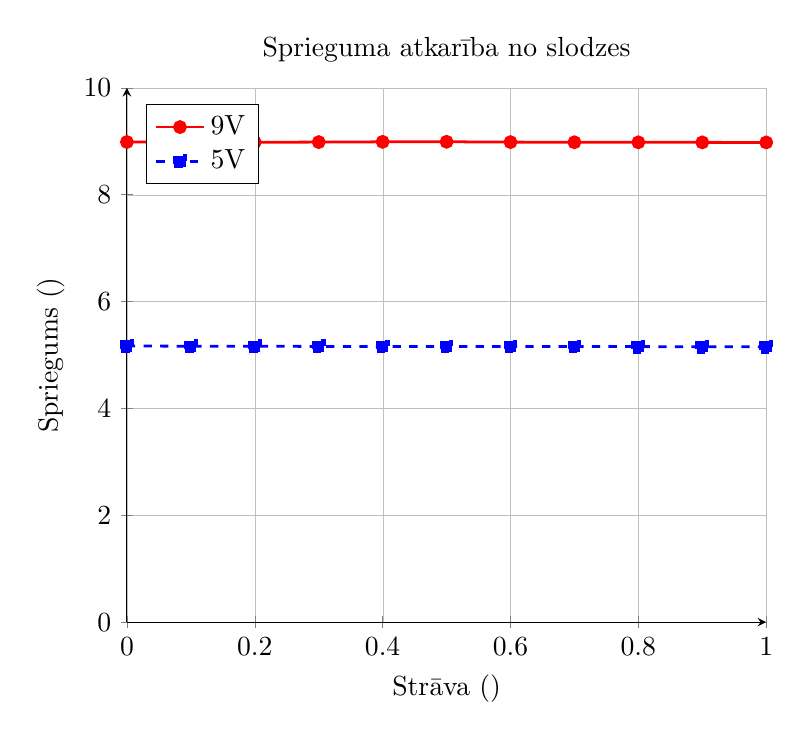
\begin{tikzpicture}
\begin{axis}[
    title={Sprieguma atkarība no slodzes},
    xlabel={Strāva (\si{\ampere})},
    ylabel={Spriegums (\si{\volt})},
    xmin=0, xmax=1,
    ymin=0, ymax=10,
    grid=both,
    grid style={line width=0.1pt, draw=gray!50},
    width=0.8\textwidth,
    axis lines=left,
    legend pos=north west,
]

% Line 1: 9V (Red)
\addplot[
    color=red,
    mark=*,
    line width=1pt,
]
coordinates {
    (0, 8.987)
    (0.1, 8.985)
    (0.2, 8.983)
    (0.3, 8.985)
    (0.4, 8.990)
    (0.5, 8.991)
    (0.6, 8.985)
    (0.7, 8.982)
    (0.8, 8.981)
    (0.9, 8.980)
    (1, 8.979)
};
\addlegendentry{9V}

% Line 2: 5V (Blue)
\addplot[
    color=blue,
    mark=square*,
    dashed,
    line width=1pt,
]
coordinates {
    (0, 5.168)
    (0.1, 5.165)
    (0.2, 5.163)
    (0.3, 5.161)
    (0.4, 5.160)
    (0.5, 5.160)
    (0.6, 5.159)
    (0.7, 5.158)
    (0.8, 5.157)
    (0.9, 5.155)
    (1, 5.153)
};
\addlegendentry{5V}

\end{axis}
\end{tikzpicture}
\caption{Strāvas-sprieguma raksturlīkne 9V un elektrobarošanas līnijām}
\end{figure}
Grafiski atveidoti iegūtie rezultāti. Maksimālais strāvas patēriņš 9 V līnijai ir 310 mA un 5 V līnijai 110 mA.
\section{True RMS jaudas detektora un RF kabeļu tests}
S-parametru noteikšanai tiek veikti no 6.5 līdz 8.5 GHz diapozonā. Tiek veikts koaksiālo kabeļu RFC1 un RFC2 S-parametru (skat. att. 2.1.), kas savieno atzarotāja $P_{fwd}$ un $P_{ref}$ ar jaudas detektoru un jaudas detektora novērtējums. Tad jaudas detektora izejas sprieguma atkarība no ieejas signāla jaudas pie 7.2 GHz.
\begin{figure}[H]
	\centering
    \includegraphics[width=0.7\textwidth]{pictures/cable_coax_fwd.jpg}\hspace{1cm}
    \caption{Izstarotās jaudas koaksiālais kabeļa S-parametri}
\end{figure}
Lielākā daļa no ienākošās jaudas koaksiālajā kabelī netiek atstarota ($S_{11}$ un $S_{22}$) atpakaļ -24 dB, kas ir aptuveni 0.4\% no jaudas, bet, neskatoties uz to, pašā vadā ir -1.8 dB zudums ($S_{21}$ un $S_{12}$), kas ir aptuveni 33\% no ienākošās jaudas.
\begin{figure}[H]
	\centering
    \includegraphics[width=0.7\textwidth]{pictures/cable_coax_ref.jpg}\hspace{1cm}
    \caption{Atstarotās jaudas koaksiālais kabelā S-parametri}
\end{figure}
Lielākā daļa no ienākošās jaudas koaksiālajā kabelī netiek atstarota ($S_{11}$ un $S_{22}$) atpakaļ -20 dB, kas ir aptuveni 1\% no jaudas, bet, neskatoties uz to, pašā kabelī ir -1.9 dB zudums ($S_{21}$ un $S_{12}$), kas ir aptuveni 36\% no ienākošās jaudas.
\begin{figure}[H]
	\centering
    \includegraphics[width=0.7\textwidth]{pictures/tests_diagram3.png}\hspace{1cm}
    \caption{Jaudas detektora testu diagramma}
\end{figure}
3.14. att. redzams testa iekārtu slēgums elektriski principiālajā shēmā.
\begin{figure}[H]
	\centering
    \includegraphics[width=0.7\textwidth]{pictures/vna_measurement_powerdet.jpeg}\hspace{1cm}
    \caption{S-parametri jaudas detektoram}
\end{figure}
Izstarotā un atstarotā jaudas kanāli atstaro aptuveni pusi no ienākošā signāla jaudas. Savstarpējā portu izolācija ir laba, kas tiek panākta ar metalizētiem urbumiem.
\begin{figure}[H]
\centering
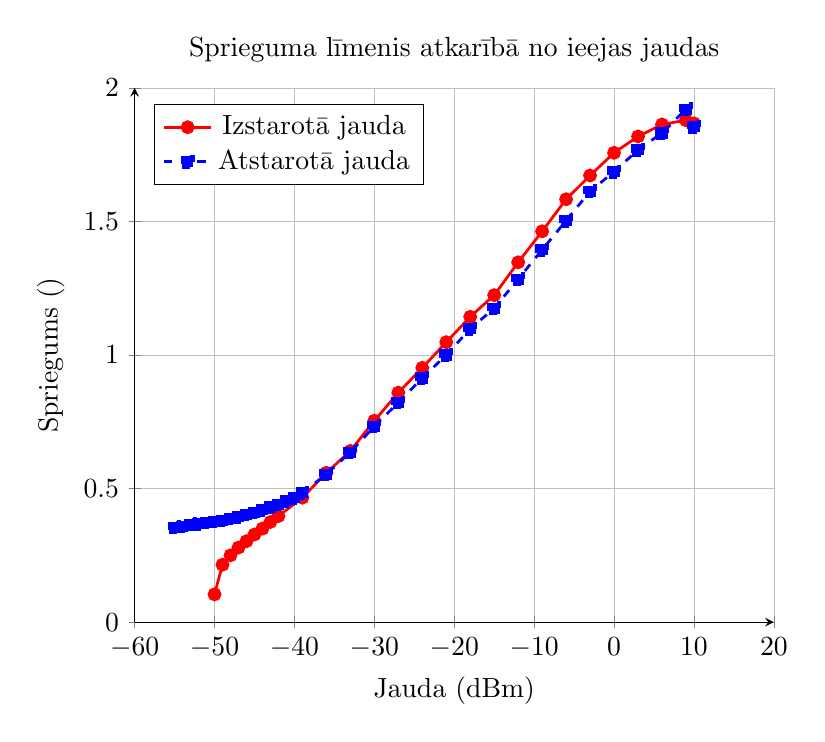
\begin{tikzpicture}
\begin{axis}[
    title={Sprieguma līmenis atkarībā no ieejas jaudas},
    xlabel={Jauda (dBm) },
    ylabel={Spriegums (\si{\volt})},
    xmin=-60, xmax=20,
    ymin=0, ymax=2,
    grid=both,
    grid style={line width=0.1pt, draw=gray!50},
    width=0.8\textwidth,
    axis lines=left,
    legend pos=north west,
]

% Line 1: FWD power (Red)
\addplot[
    color=red,
    mark=*,
    line width=1pt,
]
coordinates {
    (-50, 0.104)
    (-49, 0.215)
    (-48, 0.250)
    (-47, 0.279)
    (-46, 0.303)
    (-45, 0.328)
    (-44, 0.350)
    (-43, 0.375)
    (-42, 0.397)
    (-39, 0.466)
    (-36, 0.559)
    (-33, 0.641)
    (-30, 0.754)
    (-27, 0.859)
    (-24, 0.952)
    (-21, 1.048)
    (-18, 1.143)
    (-15, 1.224)
    (-12, 1.347)
    (-9, 1.463)
    (-6, 1.583)
    (-3, 1.672)
    (0, 1.757)
    (3, 1.818)
    (6, 1.863)
    (9, 1.879)
    (10, 1.867)
};
\addlegendentry{Izstarotā jauda}

% Line 2: REF power (Blue)
\addplot[
    color=blue,
    mark=square*,
    dashed,
    line width=1pt,
]
coordinates {
    (-55, 0.355)
    (-54, 0.358)
    (-53, 0.366)
    (-52, 0.368)
    (-51, 0.373)
    (-50, 0.377)
    (-49, 0.382)
    (-48, 0.388)
    (-47, 0.394)
    (-46, 0.403)
    (-45, 0.412)
    (-44, 0.420)
    (-43, 0.431)
    (-42, 0.442)
    (-41, 0.454)
    (-40, 0.466)
    (-39, 0.484)
    (-36, 0.554)
    (-33, 0.636)
    (-30, 0.733)
    (-27, 0.822)
    (-24, 0.914)
    (-21, 1.000)
    (-18, 1.098)
    (-15, 1.175)
    (-12, 1.284)
    (-9, 1.394)
    (-6, 1.503)
    (-3, 1.613)
    (0, 1.686)
    (3, 1.768)
    (6, 1.831)
    (9, 1.920)
    (10, 1.855)
};
\addlegendentry{Atstarotā jauda}

\end{axis}
\end{tikzpicture}
\caption{Izejas sprieguma ietekme uz ieejas jaudu}
\end{figure}
Iegūstot izejas sprieguma līmeņu atkarības no ieejas jaudas, tika ņemti vērā signāla ģeneratora un vada zudumi. Līkne, kas tika iegūta abos kanālos, ir ļoti līdzīga ražotāja dotajai specifikācijai. Jutības diapazons ir no -50 līdz 9 dBm, kur 0 dBm atbilst 100 W, tad mēs varam izmērīt no 1 mW līdz 794,3 W.
\section{Tīkla testi}
Šajā testā tiek pārbaudīta vadības sistēma no operatora datora līdz mikrokontrolieram ar skripta palīdzību, kas rakstīts Python priekš Windows OS. Tests tika veikts izolētā tīklā, kur atradās tikai divas ierīces: operātora dators un mikrokontrolieris ar visu X-joslas sistēmu.
\begin{figure}[H]
	\centering
    \includegraphics[width=0.9\textwidth]{pictures/script_start.png}\hspace{1cm}
    \caption{Klienta konfigurēšana lokālajā tīklā}
\end{figure}
Tests sākās ar skripta uzsākšanu. Terminālī redzams logo, palīgrinda un to, ka veiksmīgi ir pieslēdzies pie TCP servera, kurš uzreiz pēc pieslēgšanās atsūta savu nosaukumu un versiju. Tad lietotājam tiek sniegta informācija par komandu, kura uzsāk monitorēšanu un darba punkta iestatīšanu. Pēc tā tiek aicināts ievadīt komandu.
\begin{figure}[H]
	\centering
    \includegraphics[width=0.9\textwidth]{pictures/script_monchange.png}\hspace{1cm}
    \caption{Monitorēšanas cikla aizkaves maiņa}
\end{figure}
Redzams monitorēšanas intervāla iestatīšanu no noklusētās vērtības 30 sec uz 5 sekundēm.
\begin{figure}[H]
	\centering
    \includegraphics[width=0.9\textwidth]{pictures/script_system_start .png}\hspace{1cm}
    \caption{Darba punkta iestatīšana un telemetrijas virkne}
\end{figure}
Tad tika uzsākta sistēmas darbība ar komandu "start", kur var redzēt, ka tika nosūtīta komanda pon=1 un saņemta atbilde no mikrokontroliera pon=1, kas liecina par to, ka komanda tika saņemta un veiksmīgi apstrādāta. Pēc kā seko monitorēšanas telemetrijas ik pēc 5 sekundēm.
\begin{figure}[H]
	\centering
    \includegraphics[width=0.9\textwidth]{pictures/script_setcurr.png}\hspace{1cm}
    \caption{Darba punkta noteces strāvas iestatīšana}
\end{figure}
\begin{figure}[H]
Tad tiek iestatīts cita darba punkta strāva no 3 A uz 2.45 A, kur mikrokontrolieris arī deva atbildi, ka tā tika veiksmīgi uzstādīta.
	\centering
    \includegraphics[width=0.9\textwidth]{pictures/script_setcurr_tel.png}\hspace{1cm}
    \caption{Strāvas maiņas telemetrijas virkne}
\end{figure}
Tad var redzēt, ka telemetrijas virknē ir aizvara spriegums cits un noteces strāva 2.426 A.
\begin{figure}[H]
	\centering
    \includegraphics[width=0.9\textwidth]{pictures/script_system_stop.png}\hspace{1cm}
    \caption{Darba punkta atiestatīšana}
\end{figure}
Aktīvu sistēmu var deaktivizēt ar komandas nosūtīšanu "stop", kas uzreiz uz mikrokontrolieri nosūta komandu pon=0 un izbeidz monitorēšanas pavedienu.
\begin{figure}[H]
	\centering
    \includegraphics[width=0.9\textwidth]{pictures/script_exit.png}\hspace{1cm}
    \caption{Skripta izslēgšana}
\end{figure}
Ar exit vai ctrl+c var izbeigt skripta darbību, kur tiek aizsūtīta komanda pon=0, lai izslēgtu sistēmu, ja tā bija aktīva, un atvienojas no servera, tad izbeidz visu aktīvo pavedienu darbību.

